%%%%%%%%%%%%%%%%%%%%%%%%%%%%%%%%%%%%%%%%%%%%%%%%%%%%%%%%%%%%%%%%%%%%%%%%%%%
% Relational algebra & relational calculus for Sailer-Reserve-Boat
% schema in the DBMS book.
% Author: Shuo Yang
%%%%%%%%%%%%%%%%%%%%%%%%%%%%%%%%%%%%%%%%%%%%%%%%%%%%%%%%%%%%%%%%%%%%%%%%%%%

\documentclass[10pt]{article}
\usepackage{amsmath,amssymb,epsfig,graphics,hyperref,amsthm,mathtools}
\DeclarePairedDelimiter\ceil{\lceil}{\rceil}
\DeclarePairedDelimiter\floor{\lfloor}{\rfloor}

\hypersetup{colorlinks=true}

\setlength{\textwidth}{7in}
\setlength{\topmargin}{-0.575in}
\setlength{\textheight}{9.25in}
\setlength{\oddsidemargin}{-.25in}
\setlength{\evensidemargin}{-.25in}

\reversemarginpar
\setlength{\marginparsep}{-15mm}

\newcommand{\rmv}[1]{}
\newcommand{\bemph}[1]{{\bfseries\itshape#1}}
\newcommand{\N}{\mathbb{N}}
\newcommand{\Z}{\mathbb{Z}}
\newcommand{\imply}{\to}
\newcommand{\bic}{\leftrightarrow}

\def\Author{Shuo Yang}

\begin{document}

\noindent

\begin{center}
  Safari Queries\\
  \Author\\
\end{center}

% A horizontal split line
\hrule\smallskip

\vspace{1em}
\underline{Schema}:
\vspace{1em}

sale (\underline{sale\#}, saleqty, itemno, dname)

supplier (\underline{spl\#}, splname)

item (\underline{item\#}, itemname, itemtype, itemcolor)

department (\underline{deptname}, deptfloor, deptphone, empno)

delivery (\underline{del\#}, delqty, itemnum, dptname, splno)

employee (\underline{emp\#}, empfname, empsalary, departname, bossno)

\vspace{1em}

\underline{ER Diagram}:
\begin{center}
  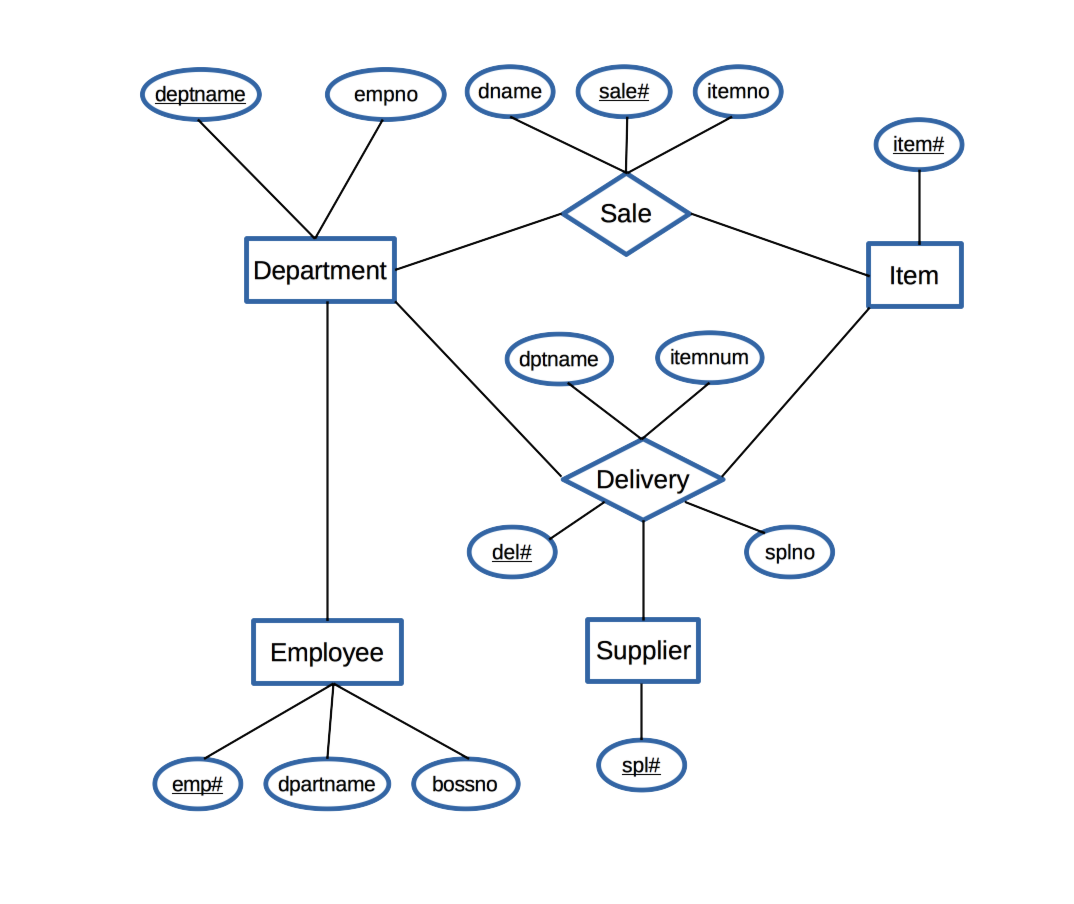
\includegraphics[width=12cm,height=10cm]{./safari-ER.png}
\end{center}

\underline{Relationships}:\\
\textbf{Supplier} \emph{delivers} \textbf{Item} to
\textbf{Department}. (many to many)\\
\textbf{Department} \emph{sells} \textbf{Item}. (many to many)\\
\textbf{Employee} \emph{manages} \textbf{Employee}. (one to many)\\
\textbf{Employee} \emph{works at} \textbf{Department}. (many to one)\\
\textbf{Department} \emph{is managed by} \textbf{Employee}. (one to one)\\

\vspace{1em}

\begin{enumerate}
\item What are the names of the suppliers?
  \begin{align*}
    \pi_{splname}(supplier)
  \end{align*}
  LEAP Query:\\
  q1r1 = project (supplier) (splname)

\item What are the names of the employees in Marketing?
  \begin{align*}
    \pi_{empfname}(\sigma_{departname='Marketing'}(employee))
  \end{align*}

  LEAP Query:\\
  q2r1 = select (employee) (departname=``Marketing'')\\
  q2r2 = project (q2r1) (empfname)

\item What is the Cartesian Product of the suppliers' names and the
  departments' names?

  \begin{align*}
    \pi_{splname}(supplier) \times \pi_{deptname}(department)
  \end{align*}

  LEAP Query:\\
  q3r1 = (project (supplier) (splname)) product (project (department)
  (deptname))

\item What are the item numbers of the items sold by the departments
  located on the second floor? (You must not use JOIN for this query)

  \begin{align*}
    \pi_{itemno}(\sigma_{dname=deptname}(sale \times
    (\sigma_{deptfloor=2}(department))))
  \end{align*}

  LEAP Query:\\
  q4r1 = (sale) product (department)\\
  q4r2 = select (q4r1) (dname=deptname)\\
  q4r3 = select (q4r2) (deptfloor='2')\\
  q4r4 = project (q4r3) (itemno)

\item What are the item numbers of the items sold by the departments
  located on the second floor? (You must use JOIN for this query)

  \begin{align*}
    \pi_{itemno}(\sigma_{deptfloor=2}(department)
    \bowtie_{deptname=dname} sale)
  \end{align*}

  LEAP Query:\\
  q5r1 = join (department) (sale) (deptname=dname)\\
  q5r2 = project (select (q5r1) (deptfloor='2')) (itemno)

\item For each item, give its type, the departments that sell it, and
  the floor number of these departments.

  \begin{align*}
    \pi_{item\#, itemtype, dname, deptfloor}((item
    \bowtie_{item\#=itemno} sale) \bowtie_{dname=deptname} department)
  \end{align*}

  LEAP Query:\\
  q6r1 = join (item) (sale) (item\#=itemno)\\
  q6r2 = join (q6r1) (department) (dname=deptname)\\
  q6r3 = project (q6r2) (itemno, itemtype, dname, deptfloor)

\item List the numbers of the items delivered by Nepalese Corp or sold
  in the Navigation department.

  \begin{align*}
    (\pi_{itemno}(\sigma_{dname='Navigation'}sale)) \cup
    (\pi_{itemnum}(\sigma_{splname='Nepalese\_Corp'}supplier
    \bowtie_{spl\#=splno} delivery))
  \end{align*}

  LEAP Query:\\
  q7r1 = project (select (sale) (dname=``Navigation'')) (itemno)\\
  q7r2 = join (select (supplier) (splname=``Nepalese\_Corp''))
  (delivery) (spl\#=splno)\\
  q7r3 = project (q7r2) (itemnum)\\
  q7r4 = (q7r1) union (q7r3)

\item What are the names of the items sold on floors other than the
  second floor?

  \begin{align*}
    &\rho(TmpItem, \pi_{itemno}(sale \bowtie (\sigma_{deptfloor \neq
      2}department)))\\
    &\pi_{itemname}(TmpItem \bowtie_{itemno=item\#} item)
  \end{align*}

  LEAP Query:\\
  q8r1 = select (department)(deptfloor $<>$ '2')\\
  q8r2 = join (q8r1) (sale) (deptname = dname)\\
  q8r3 = project (q8r2) (itemno)\\
  q8r4 = join (q8r3) (item) (itemno = item\#)\\
  q8r5 = project (q8r4) (itemname)

\item Find the names of the items sold by no department on the second
  floor.

  \begin{align*}
    &\rho(TmpItem1, \pi_{itemno}(sale \bowtie (\sigma_{deptfloor =
      2}department)))\\
    &\rho(TmpItem2, (\sigma_{itemno}sale) - TmpItem1)\\
    &\pi_{itemname}(TmpItem2 \bowtie item)
  \end{align*}

  LEAP Query:\\
  q9r1 = join (select (department) (deptfloor='2')) (sale)
  (deptname=dname)\\
  q9r2 = (project (sale) (itemno)) difference (project (q9r1)
  (itemno))\\
  q9r3 = project (join (q9r2) (item) (item\# = itemno)) (itemname)

\item List the item numbers of the items delivered by Nepalese Corp
  and sold in the Navigation department. (You must use $\cap$)

  \begin{align*}
    (\pi_{itemno}(\sigma_{dname='Navigation'}sale)) \cap
    (\pi_{itemnum}(\sigma_{splname='Nepalese\_Corp'}supplier
    \bowtie_{spl\#=splno} delivery))
  \end{align*}

  LEAP Query:\\
  q10r1 = project (select (sale) (dname=``Navigation'')) (itemno)\\
  q10r2 = join (select (supplier) (splname=``Nepalese\_Corp''))
  (delivery) (spl\#=splno)\\
  q10r3 = project (q10r2) (itemnum)\\
  q10r4 = (q10r1) intersect (q10r3)

\item What are the names of the suppliers of Pith helmets sold in a
  department managed by Andrew?

  \begin{align*}
    &\rho(TmpDep, department \bowtie
    \sigma_{empfname='Andrew'}employee)\\
    &\rho(TmpSale, sale \bowtie
    \sigma_{itemname='Pith\_helmet'}item)\\
    &\rho(TmpDepSale, TmpDep \bowtie TmpSale)\\
    &\rho(TmpDelivery, delivery \bowtie
    \sigma_{itemname='Pith\_helmet'}item)\\
    &\rho(TmpDelSup, TmpDelivery \bowtie supplier)\\
    &\pi_{splname}(TmpDepSale_{dptname=dname} \bowtie TmpDelSup)
  \end{align*}

  LEAP Query:\\
  q11r1 = join (department) (select (employee)
  (empfname=``Andrew'')) (empno = emp\#)\\
  q11r2 = join (sale) (select (item) (itemname=``Pith\_helmet''))
  (itemno = item\#)\\
  q11r3 = join (q11r1) (q11r2) (dname=deptname)\\
  q11r4 = join (delivery) (select (item) (itemname=``Pith\_helmet''))
  (itemnum = item\#)\\
  q11r5 = join (q11r4) (supplier) (splno = spl\#)\\
  q11r6 = join(q11r5) (q11r3) (dptname=deptname) \\
  q11r7 = project (q11r6) (splname)

\item What are the item numbers of the items sold by all departments
  on the second floor? (You must use division)

  \begin{align*}
    &\rho(TmpDep, \pi_{deptname}(\sigma_{deptfloor=2}department))\\
    &\rho(TmpSale, \pi_{itemno, dname}(sale))\\
    &TmpSale - ((\pi_{item\#}item \times TmpDep) - TmpSale)
  \end{align*}

  q12r1 = project (select (department) (deptfloor='2')) (deptname)\\
  q12r11 = join (sale) (q12r1) (deptname=dname)\\
  q12r2 = project (q12r11) (itemno, dname)\\
  q12r3 = project (item) (item\#)\\
  q12r4 = ((q12r3) product (q12r1)) difference (q12r2)\\
  q12r5 = (project (q12r2) (itemno)) difference (project (q12r4) (itemno))

\end{enumerate}
\end{document}
